\section{第六周数值分析实验}
\subsection{Bernstein多项式}
\begin{definition}
	设$f:[0,1]\to\mathbb{R}$,称
	$$
	B_n(f;x)=\sum_{i=0}^{n}f\left(\frac{i}{n}\right)B_i^n(x),x\in[0,1]
	$$
	为$f$的$n$次Bernstein多项式,其中$B_i^n(x)=\binom{n}{i}x^i(1-x)^{n-i}$.
\end{definition}
\lstinputlisting[language=matlab]{day5/bernstein_n.m}
\begin{ex}
	当$f(x)=\cos 2\pi x$时,分别给出$n=3, 5, 7, 9, 10$时的$B_n(f,x)$表达式,并绘制$f(x)$与$B_n(f,x)$的图像.
\end{ex}
\lstinputlisting[language=matlab]{day5/work6.m}
\begin{figure}[H]
	\centering
	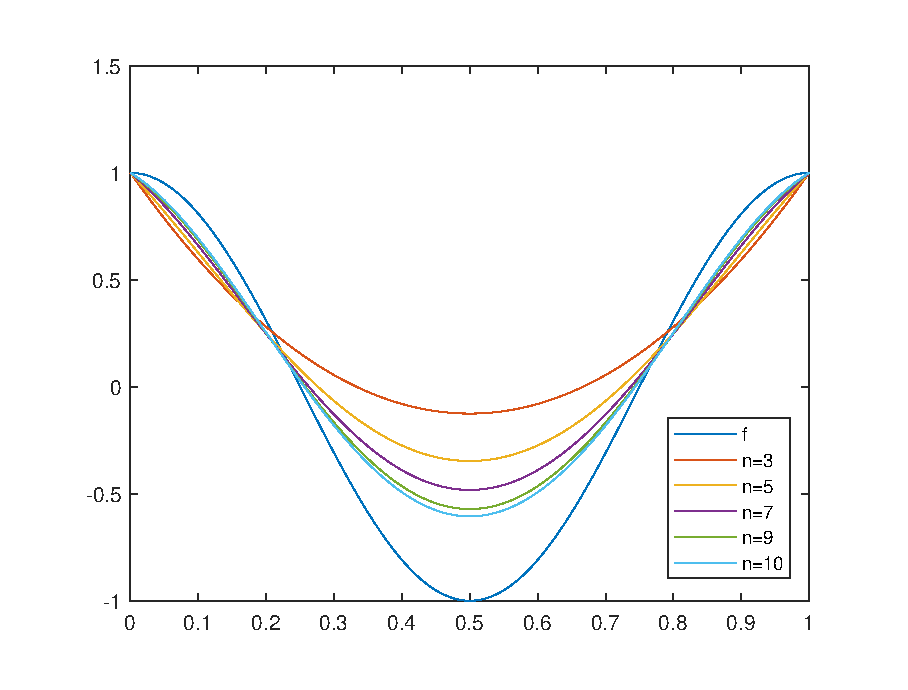
\includegraphics[width = 0.6\linewidth]{day5/fig.eps}
	\caption{Bernstein多项式图像}
\end{figure}